\documentclass[solutionorbox,answers]{exam}
% \documentclass[solutionorbox]{exam}

%%%%%%%%%%%%%%%%%%%%%%%%%%%%%%%%%%%%%%%%%%%%%%%%%%%%%%%%%%%%%%%
% Update to change header
\newcommand{\courseName}{CS 577}
\newcommand{\assignmentName}{Assignment 1 -- Discrete Review}
\newcommand{\semester}{Spring 2023}
%%%%%%%%%%%%%%%%%%%%%%%%%%%%%%%%%%%%%%%%%%%%%%%%%%%%%%%%%%%%%%%

\usepackage[utf8]{inputenc}
\usepackage[T1]{fontenc}

\usepackage{amsmath}
\usepackage{amsfonts}
\usepackage{amsthm}
\usepackage{amssymb}
\usepackage{booktabs}
\usepackage{forest}
\usepackage{xcolor}
\usepackage{tkz-graph}
\usepackage[ruled]{algorithm2e}
\usepackage{graphicx}
\usepackage{multicol}

\usepackage{listings}
\lstset{basicstyle=\ttfamily,
  showstringspaces=false,
  commentstyle=\color{red},
  keywordstyle=\color{blue}
}

\usepackage{hyperref}

\pagestyle{headandfoot}
\runningheadrule
\firstpageheader{\courseName}{\huge \assignmentName}{\semester}
\runningheader{\courseName}
{\assignmentName}
{\semester}
\firstpagefooter{}{}{}
\runningfooter{}{Page \thepage\ of \numpages}{}

\begin{document}

\begin{center}
\fbox{\parbox{5.5in}{\centering
Answer the questions in the boxes provided on the
question sheets. If you run out of room for an answer,
add a page to the end of the document. \\
\vspace{0.1in}
Related Readings: \url{http://pages.cs.wisc.edu/~hasti/cs240/readings/}
}}
\end{center}
\vspace{0.1in}
\makebox[0.48\textwidth]{Name:\enspace KJ Choi} \qquad
\makebox[0.48\textwidth]{Wisc id:\enspace 908 028 9540}

\begin{questions}

\section*{Logic}

  \question
  Using a truth table, show the equivalence of the following statements.
\begin{parts}
  \part
  $P \vee (\neg P \wedge Q) \equiv P \vee Q$
  \nopagebreak
  \begin{solutionbox}{2in}\\

    \begin{tabular}{ |c|c|c|c|c|c| } 
      \hline
      $P$ & $Q$ & $\neg P$ & $\neg P \wedge Q$ & $P \vee (\neg P \wedge Q)$ & $P \vee Q$ \\ 
      \hline
      T & T & F & F & T & T \\ 
      \hline
      T & F & F & F & T & T \\ 
      \hline
      F & T & T & T & T & T \\ 
      \hline
      F & F & T & F & F & F\\ 
      \hline
    \end{tabular}
  
  \end{solutionbox}
  
  \part
  $\neg P \vee \neg Q \equiv \neg (P \wedge Q)$
  \nopagebreak
  \begin{solutionbox}{2in}\\

    \begin{tabular}{ |c|c|c|c|c|c|c| }  
      \hline
      $P$ & $Q$ & $\neg P$ & $\neg Q$ & $ P \wedge Q$ & $\neg P \vee \neg Q$ & $\neg (P \wedge Q)$ \\ 
      \hline
      T & T & F & F & T & F & F \\ 
      \hline
      T & F & F & T & F & T & T \\ 
      \hline
      F & T & T & F & F & T & T \\ 
      \hline 
      F & F & T & T & F & T & T \\ 
      \hline
    \end{tabular}
    
  \end{solutionbox}
  
  \part
  $\neg P \vee P \equiv \text{true}$
  \nopagebreak
  \begin{solutionbox}{2in} \vspace{1em} \\

    \begin{tabular}{ |c|c|c|c| }  
      \hline
      $P$ & $\neg P$ & $\neg P \vee P$& True \\ 
      \hline
      T & F & T & T\\ 
      \hline
      F & T & T & T\\ 
      \hline
    \end{tabular}

  \end{solutionbox}
  
  \part
  $P \vee (Q \wedge R) \equiv (P \vee Q) \wedge (P \vee R)$
  \nopagebreak
  \begin{solutionbox}{3in}\\
    
    \begin{tabular}{ |c|c|c|c|c|c|c|c| }  
      \hline
      $P$ & $Q$ & $R$ & $Q \wedge R$ & $P \vee Q$ & $P \vee R$ & $P \vee (Q \wedge R)$ & $(P \vee Q) \wedge (P \vee R)$\\ 
      \hline
      T & T & T & T & T & T & T & T\\
      \hline
      T & T & F & F & T & T & T & T\\
      \hline
      T & F & T & F & T & T & T & T\\
      \hline
      T & F & F & F & T & T & T & T\\
      \hline
      F & T & T & T & T & T & T & T\\
      \hline
      F & T & F & F & T & F & F & F\\
      \hline
      F & F & T & F & F & T & F & F\\
      \hline
      F & F & F & F & F & F & F & F\\
      \hline
    \end{tabular}

  \end{solutionbox}
  
\end{parts}

\newpage
\section*{Sets}


  \question
  Based on the definitions of the sets $A$ and $B$, calculate the following: $|A|$, $|B|$, $A \cup B$, $A \cap B$, $A \setminus B$, $B \setminus A$.

  \begin{parts}
    \part
    $A = \{1, 2, 6, 10\}$ and $B = \{2, 4, 9, 10\}$
    \nopagebreak
    \begin{solutionbox}{2in}

      $|A| = 4$ \\
      $|B| = 4$ \\
      $A \cup B = \{1, 2, 4, 6, 9, 10\}$ \\
      $A \cap B = \{2, 10\}$ \\
      $A \setminus B = \{1, 6\}$ \\
      $B \setminus A = \{4, 9\}$ \\

    \end{solutionbox}
    \part
    $A = \{x \mid x \in \mathbb{N}\}$ and $B = \{x \in \mathbb{N} \mid x \text{ is even} \}$
    \nopagebreak
    \begin{solutionbox}{2in}
      
      $|A| = \infty$ \\
      $|B| = \infty$ \\
      $A \cup B = \{x \mid x \in \mathbb{N}\}$ \\
      $A \cap B = \{x \in \mathbb{N} \mid x \text{ is even} \}$ \\
      $A \setminus B = \{x \in \mathbb{N} \mid x \text{ is odd} \}$ \\
      $B \setminus A = \varnothing$ \\

    \end{solutionbox}

  \end{parts}

\section*{Relations and Functions}

\question
For each of the following relations, indicate if it is reflexive, antireflexive, symmetric, antisymmetric, or transitive.

\begin{parts}
\part
$\{(x,y) : x \le y\}$
\begin{solutionbox}{0.5in}

  reflexive, transitive

\end{solutionbox}
\part
$\{(x,y) : x > y\}$
\begin{solutionbox}{0.5in}

  antireflexive, transitive

\end{solutionbox}
\newpage
\part
$\{(x,y) : x < y\}$
\begin{solutionbox}{0.5in}
  antireflexive, transitive
\end{solutionbox}
\part
$\{(x,y) : x = y\}$ 
\begin{solutionbox}{0.5in}
  reflexive, symmetric, transitive
\end{solutionbox}
\end{parts}

\question
For each of the following functions (assume that they are all $f: \mathbb{Z} \to \mathbb{Z}$), indicate if it is surjective (onto), injective (one-to-one), or bijective.

\begin{parts}
\part
$f(x) = x$
\begin{solutionbox}{0.5in}
  bijective
\end{solutionbox}
\part
$f(x) = 2x - 3$
\begin{solutionbox}{0.5in}
  bijective
\end{solutionbox}
\part
$f(x) = x^2$
\begin{solutionbox}{0.5in}
  onto
\end{solutionbox}
\end{parts}
\question
Show that $h(x) = g(f(x))$ is a bijection if $g(x)$ and $f(x)$ are bijections.

\begin{solutionbox}{3in}
  
  In order to prove $h(x) = g(f(x))$ is a bijection function given that $g(x)$ and $f(x)$ are bijections, we need to prove that the function is injective (i) and surjective (ii).\\ 
  \\
  To prove the the function is injective (i), we must prove that $(\forall a_1, a_2) h(a_1)=h(a_2) \rightarrow a_1=a_2$.\\
  We can rewrite the statement $h(a_1)=h(a_2)$ as $g(f(a_1))=g(f(a_2))$.\\
  Since $g$ and $f$ are bijective, $g(f(a_1))=g(f(a_2)) \Rightarrow f(a_1)=f(a_2) \rightarrow a_1 = a_2$.\\
  Thus, $(\forall a_1, a_2) h(a_1)=h(a_2) \rightarrow a_1=a_2$ is true, i.e. $h(x)$ is injective.\\
  \\
  To prove the the function is surjective (ii), we must prove that $(\forall c \in C)(\exists a \in A)(h(a)=g(f(a))=c)$, given that $C$ and $A$ are domain and range of the function $h(x)$.\\
  Let $f:A \rightarrow B$ and $g:B \rightarrow C$. Since $f$ and $g$ are bijective, $(\forall b \in B)(\exists! a \in A)(f(a))=b)$ and $(\forall c \in C)(\exists! b \in B)(g(b))=c)$. 
  This implies $(\forall c \in C)(\exists! a \in A)(h(a)=g(f(a))=c)$.\\
  Thus, $(\forall c \in C)(\exists a \in A)(h(a)=c)$ holds true, i.e. $h(x)$ is surjective.\\
  \\
  Since $h(x)$ is both injective (i) and surjective (ii), $h(x)$ is bijective.
  
\end{solutionbox}

\section*{Induction}
\label{sec:induction}

\question
Prove the following by induction.

\begin{parts}
  \part
  $\sum_{i = 1}^n i = n(n+1)/2$
  \begin{solutionbox}{2.3in}\\
    We use induction to show that $P(n)$ holds for all natural numbers $n \geq 1$ where\\
    $P(n) : \sum_{i=1}^{n} i = n(n+1)/2$\\

    Base case: $P(1) : \sum_{i=1}^{1} i = 1$ and $1(1+1)/2 = 1$. So, $P(1)$ holds.\\

    Inductive case:
    IH: $P(k)$ holds, i.e. $\sum_{i=1}^{k} i = k(k+1)/2$\\
    Now consider $P(k+1) : \sum_{i=1}^{k+1}i=\sum_{i=1}^{k}i+(k+1)=k(k+1)/2+(k+1)$\\
    by induction hypothesis.\\
    $k(k+1)/2+(k+1) = (k+1)(k+2)/2 = (k+1)((k+1)+1)/2$.
    Thus, $P(k+1)$ holds.\\
    
    Therefore, by induction, $P(n)$ holds for all natural number $n \geq 1$. 

  \end{solutionbox}

  \part
  $\sum_{i = 1}^n i^2 = n(n+1)(2n+1)/6$
  \begin{solutionbox}{2.3in}\\
    Let $P(n) : \sum_{i = 1}^n i^2 = n(n+1)(2n+1)/6$ for all natural numbers $n \geq 1$.\\

    Base case: $P(1) : \sum_{i=1}^{1} i^2 = 1$ and $1(1+1)(2*1+1)/6 = 6/6 = 1$. So, $P(1)$ holds.\\

    Inductive case:
    IH: $P(k)$ holds, i.e. $\sum_{i=1}^{k} i^2 = k(k+1)(2k+1)/6$\\
    Now consider $P(k+1) : \sum_{i=1}^{k+1}i^2=\sum_{i=1}^{k}i^2+(k+1)^2=k(k+1)(2k+1)/6+(k+1)^2$\\
    by induction hypothesis.\\
    $k(k+1)(2k+1)/6+(k+1)^2 = (k+1)(2k^2+7k+6)/6 = (k+1)(k+2)(2k+3)/6$\\
    $=(k+1)((k+1)+1)(2(k+1)+1)/6$. Thus, $P(k+1)$ holds.\\
    
    Therefore, by induction, $P(n)$ holds for all natural number $n \geq 1$.

  \end{solutionbox}
  
  \part
  $\sum_{i = 1}^n i^3 = n^2(n+1)^2/4$
  \begin{solutionbox}{2.4in}\\
    Let $P(n) : \sum_{i = 1}^n i^3 = n^2(n+1)^2/4$ for all natural numbers $n \geq 1$.\\

    Base case: $P(1) : \sum_{i=1}^{1} i^3 = 1$ and $1^2(1+1)^2/4 = 1$. So, $P(1)$ holds.\\

    Inductive case:
    IH: $P(k)$ holds, i.e. $\sum_{i=1}^{k} i^3 = n^2(n+1)^2/4$\\
    Now consider $P(k+1) : \sum_{i=1}^{k+1}i^3=\sum_{i=1}^{k}i^3+(k+1)^3=k^2(k+1)^2/4+(k+1)^3$\\
    by induction hypothesis.\\
    $k^2(k+1)^2/4+(k+1)^3 = (k+1)^2(k^2+4k+4)/4 = (k+1)^2(k+2)^2/4$\\
    $=(k+1)^2((k+1)+1)^2/4$\\
    Thus, $P(k+1)$ holds.\\

    Therefore, by induction, $P(n)$ holds for all natural number $n \geq 1$.
  \end{solutionbox}
\end{parts}

\section*{Graphs and Trees}
\label{sec:graphs-trees}

\question 
Give the adjacency matrix, adjacency list, edge list, and incidence matrix for the following graph. \\
\begin{minipage}{0.3\linewidth}
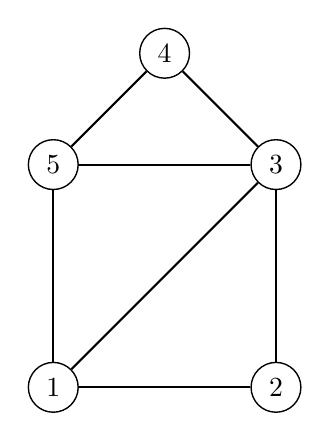
\begin{tikzpicture}
\GraphInit[vstyle=Normal]
\SetGraphUnit{2}
\begin{scope}[rotate=-135]
\Vertices{circle}{1,2,3,5}
\end{scope}
\NOEA[unit=1.414](5){4}
\Edges(1,2,3,5,4,3,1,5)
\end{tikzpicture}
\end{minipage}
\qquad
\begin{minipage}{0.6\linewidth}
\begin{solutionbox}{3.8in}\\
  adjacency matrix:
  $\begin{bmatrix}
  0 & 1 & 1 & 0 & 1 \\
  1 & 0 & 1 & 0 & 0 \\
  1 & 1 & 0 & 1 & 1 \\
  0 & 0 & 1 & 0 & 1 \\
  1 & 0 & 1 & 1 & 0
  \end{bmatrix}$\\
  \\
  adjacency list:
  \begin{tabular}{ c|l }  
    1&[2, 3, 5]\\
    2&[1, 3]\\
    3&[1, 2, 4, 5]\\
    4&[3, 5]\\
    5&[1, 3, 4]
  \end{tabular}\\
  \\
  edge list: [(1,2), (1,3), (1,5), (2,3), (3,4), (3,5), (4,5)]\\
  \\
  incidence matrix:
  $\begin{bmatrix}
    1 & 1 & 1 & 0 & 0 & 0 & 0 \\
    1 & 0 & 0 & 1 & 0 & 0 & 0 \\
    0 & 1 & 0 & 1 & 1 & 1 & 0 \\
    0 & 0 & 0 & 0 & 0 & 1 & 1 \\
    0 & 0 & 1 & 0 & 1 & 0 & 1 
    \end{bmatrix}$\\
\end{solutionbox}
\end{minipage}
\question
How many edges are there is a complete graph of size $n$? Prove by induction.

\begin{solutionbox}{3.8in}

  Let $P(n) : |E_n| =n(n-1)/2$, given $n \geq 1$ and $E$ is an edge list of a complete graph of size $n$.\\

  Base case: $P(1) : 1(1-1)/2 = 0$ and a complemte graph with single node has no edges. So $P(1)$ holds.

  Inductive case:
  IH: $P(k)$ holds, i.e. $|E_k|=k(k-1)/2$\\

  Now consider $P(k+1) : |E_k+1| = |E_k|+k = k(k-1)/2+k$ by induction hypothesis.\\
  $k(k-1)/2+k = k(k+1)/2 = (k+1)((k+1)-1)/2$\\
  Thus, $P(k+1)$ holds.\\

  Therefore, by induction, $P(n)$ holds for all natural number $n \geq 1$.

\end{solutionbox}

\question
Draw all possible (unlabelled) trees with 4 nodes.

\begin{solutionbox}{3.8in}
\\
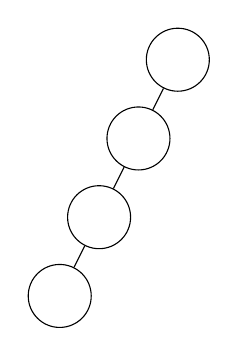
\begin{tikzpicture} 
\draw (1.5,6.0) node[minimum size=8mm,draw,circle](one) {}; 
\draw (1.0,5.0) node[minimum size=8mm,draw,circle](two) {}; 
\draw (0.5,4.0) node[minimum size=8mm,draw,circle](three) {}; 
\draw (0.0,3.0) node[minimum size=8mm,draw,circle](four) {}; 
\draw (one) -- (two);
\draw (two) -- (three);
\draw (three) -- (four);
\end{tikzpicture}
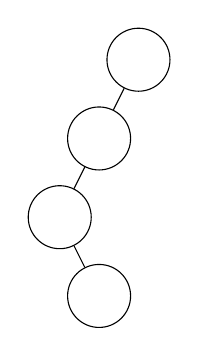
\begin{tikzpicture} 
\draw (1.5,6.0) node[minimum size=8mm,draw,circle](one) {}; 
\draw (1.0,5.0) node[minimum size=8mm,draw,circle](two) {}; 
\draw (0.5,4.0) node[minimum size=8mm,draw,circle](three) {}; 
\draw (1.0,3.0) node[minimum size=8mm,draw,circle](four) {}; 
\draw (one) -- (two);
\draw (two) -- (three);
\draw (three) -- (four);
\end{tikzpicture}
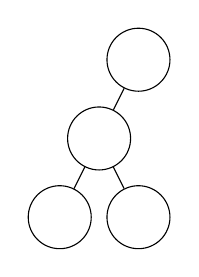
\begin{tikzpicture} 
\draw (1.5,6.0) node[minimum size=8mm,draw,circle](one) {}; 
\draw (1.0,5.0) node[minimum size=8mm,draw,circle](two) {}; 
\draw (0.5,4.0) node[minimum size=8mm,draw,circle](three) {}; 
\draw (1.5,4.0) node[minimum size=8mm,draw,circle](four) {}; 
\draw (one) -- (two);
\draw (two) -- (three);
\draw (two) -- (four);
\end{tikzpicture}
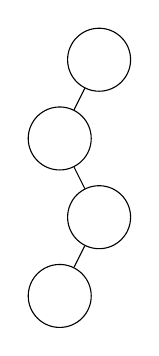
\begin{tikzpicture} 
\draw (1.5,6.0) node[minimum size=8mm,draw,circle](one) {}; 
\draw (1.0,5.0) node[minimum size=8mm,draw,circle](two) {}; 
\draw (1.5,4.0) node[minimum size=8mm,draw,circle](three) {}; 
\draw (1.0,3.0) node[minimum size=8mm,draw,circle](four) {}; 
\draw (one) -- (two);
\draw (two) -- (three);
\draw (three) -- (four);
\end{tikzpicture}
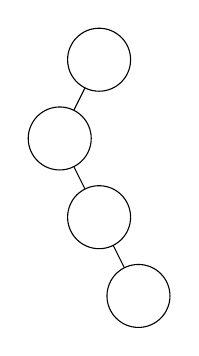
\begin{tikzpicture} 
\draw (1.5,6.0) node[minimum size=8mm,draw,circle](one) {}; 
\draw (1.0,5.0) node[minimum size=8mm,draw,circle](two) {}; 
\draw (1.5,4.0) node[minimum size=8mm,draw,circle](three) {}; 
\draw (2.0,3.0) node[minimum size=8mm,draw,circle](four) {}; 
\draw (one) -- (two);
\draw (two) -- (three);
\draw (three) -- (four);
\end{tikzpicture}
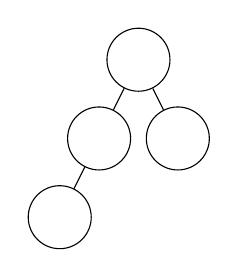
\begin{tikzpicture} 
\draw (1.5,6.0) node[minimum size=8mm,draw,circle](one) {}; 
\draw (1.0,5.0) node[minimum size=8mm,draw,circle](two) {}; 
\draw (0.5,4.0) node[minimum size=8mm,draw,circle](three) {}; 
\draw (2.0,5.0) node[minimum size=8mm,draw,circle](four) {}; 
\draw (one) -- (two);
\draw (two) -- (three);
\draw (one) -- (four);
\end{tikzpicture}
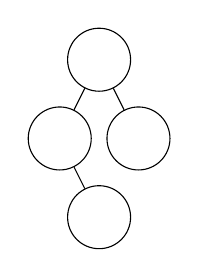
\begin{tikzpicture} 
\draw (1.5,6.0) node[minimum size=8mm,draw,circle](one) {}; 
\draw (1.0,5.0) node[minimum size=8mm,draw,circle](two) {}; 
\draw (1.5,4.0) node[minimum size=8mm,draw,circle](three) {}; 
\draw (2.0,5.0) node[minimum size=8mm,draw,circle](four) {}; 
\draw (one) -- (two);
\draw (two) -- (three);
\draw (one) -- (four);
\end{tikzpicture}\\
\\
\\
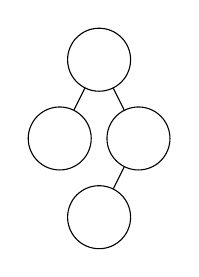
\begin{tikzpicture} 
\draw (1.5,6.0) node[minimum size=8mm,draw,circle](one) {}; 
\draw (1.0,5.0) node[minimum size=8mm,draw,circle](two) {}; 
\draw (2.0,5.0) node[minimum size=8mm,draw,circle](three) {}; 
\draw (1.5,4.0) node[minimum size=8mm,draw,circle](four) {}; 
\draw (one) -- (two);
\draw (one) -- (three);
\draw (three) -- (four);
\end{tikzpicture}
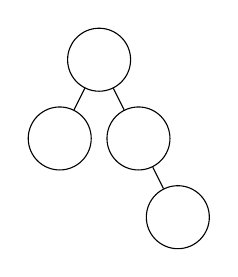
\begin{tikzpicture} 
\draw (1.5,6.0) node[minimum size=8mm,draw,circle](one) {}; 
\draw (1.0,5.0) node[minimum size=8mm,draw,circle](two) {}; 
\draw (2.0,5.0) node[minimum size=8mm,draw,circle](three) {}; 
\draw (2.5,4.0) node[minimum size=8mm,draw,circle](four) {}; 
\draw (one) -- (two);
\draw (one) -- (three);
\draw (three) -- (four);
\end{tikzpicture}
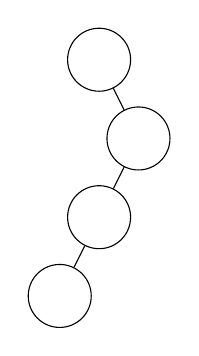
\begin{tikzpicture} 
\draw (1.5,6.0) node[minimum size=8mm,draw,circle](one) {}; 
\draw (2.0,5.0) node[minimum size=8mm,draw,circle](two) {}; 
\draw (1.5,4.0) node[minimum size=8mm,draw,circle](three) {}; 
\draw (1.0,3.0) node[minimum size=8mm,draw,circle](four) {}; 
\draw (one) -- (two);
\draw (two) -- (three);
\draw (three) -- (four);
\end{tikzpicture}
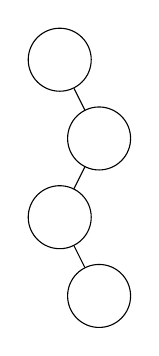
\begin{tikzpicture} 
\draw (1.5,6.0) node[minimum size=8mm,draw,circle](one) {}; 
\draw (2.0,5.0) node[minimum size=8mm,draw,circle](two) {}; 
\draw (1.5,4.0) node[minimum size=8mm,draw,circle](three) {}; 
\draw (2.0,3.0) node[minimum size=8mm,draw,circle](four) {}; 
\draw (one) -- (two);
\draw (two) -- (three);
\draw (three) -- (four);
\end{tikzpicture}
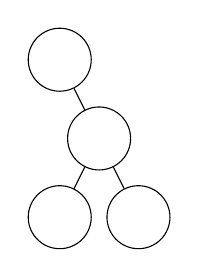
\begin{tikzpicture} 
\draw (1.5,6.0) node[minimum size=8mm,draw,circle](one) {}; 
\draw (2.0,5.0) node[minimum size=8mm,draw,circle](two) {}; 
\draw (1.5,4.0) node[minimum size=8mm,draw,circle](three) {}; 
\draw (2.5,4.0) node[minimum size=8mm,draw,circle](four) {}; 
\draw (one) -- (two);
\draw (two) -- (three);
\draw (two) -- (four);
\end{tikzpicture}
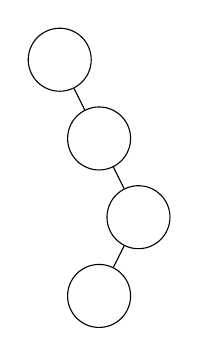
\begin{tikzpicture} 
\draw (1.5,6.0) node[minimum size=8mm,draw,circle](one) {}; 
\draw (2.0,5.0) node[minimum size=8mm,draw,circle](two) {}; 
\draw (2.5,4.0) node[minimum size=8mm,draw,circle](three) {}; 
\draw (2.0,3.0) node[minimum size=8mm,draw,circle](four) {}; 
\draw (one) -- (two);
\draw (two) -- (three);
\draw (three) -- (four);
\end{tikzpicture}
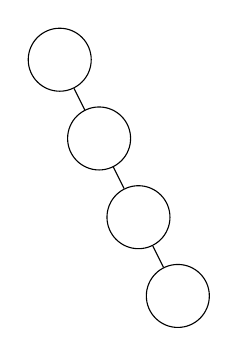
\begin{tikzpicture} 
\draw (1.5,6.0) node[minimum size=8mm,draw,circle](one) {}; 
\draw (2.0,5.0) node[minimum size=8mm,draw,circle](two) {}; 
\draw (2.5,4.0) node[minimum size=8mm,draw,circle](three) {}; 
\draw (3.0,3.0) node[minimum size=8mm,draw,circle](four) {}; 
\draw (one) -- (two);
\draw (two) -- (three);
\draw (three) -- (four);
\end{tikzpicture}
\end{solutionbox}

\question
Show by induction that, for all trees, $|E| = |V| - 1$.

\begin{solutionbox}{3.8in}

  Let $P(n):|E_n|=|V_n|-1$, given $n \geq 1$ and $E$, $V$ are list of edges and vertices of a tree with $n$ nodes.\\

  Base case: $P(1):|E_1|=|V_1|-1 = 0$. Since a tree with single node has no edges, $P(1)$ holds.

  Inductive case:
  IH: $P(k)$ holds, i.e. $|E_k|=|V_k|-1$\\

  Now consider $P(k+1) : |E_{k+1}|= |E_k|+1 = (|V_k|-1)+1 = |V_k|$ by induction hypothesis.\\
  $|V_k| = k$ and $|V_{k+1}|-1 = (k+1)-1 = k$
  Thus, $P(k+1)$ holds.\\

  Therefore, by induction, $P(n)$ holds for all natural number $n \geq 1$.

\end{solutionbox}

\section*{Counting}
\label{sec:counting}

\question
How many 3 digit pin codes are there?

\begin{solutionbox}{0.5in}
  $10^3 = 1000$
\end{solutionbox}

\question
What is the expression for the sum of the $i$th line (indexing starts at 1) of the following: \\
\begin{minipage}{0.1\textwidth}
\begin{align*}
 & 1        \\
 & 2\ 3      \\
 & 4\ 5\ 6    \\
 & 7\ 8\ 9\ 10 \\
 & \vdots
\end{align*}
\end{minipage}
\begin{minipage}{0.89\linewidth}
\begin{solutionbox}{2in} \\
    Let the sum of the $i$th line be $\sum_{k=min_i}^{max_i}k$, where $min_i$ and $max_i$ are the smallest and largest value in the $ith$ line.\\
    $min_i = (\sum_{a=1}^{i-1}a)+1 = \frac{(i-1)(i-1+1)}{2}+1 = \frac{i^2-i+2}{2}$, and\\
    $max_i = \sum_{b=1}^{i}b = \frac{i(i+1)}{2}$ by arithmetic series sum formula.\\
    $\sum_{k=min_i}^{max_i}k = i(max_i+min_i)/2 = i(\frac{i(i+1)}{2}+\frac{i^2-i+2}{2})/2 = i(i^2+1)/2$\\
    \\
    \\
    $\therefore i(i^2+1)/2$
\end{solutionbox}
\end{minipage}

\question
A standard deck of 52 cards has 4 suits, and each suit has card number 1 (ace) to 10, a jack, a queen, and a king. A standard poker hand has 5 cards. For the following, how many ways can the described hand be drawn from a standard deck.

\begin{parts}
  \part
  A royal flush: all 5 cards have the same suit and are 10, jack, queen, king, ace.
  \begin{solutionbox}{0.5in}
    
    ${4 \choose 1}=4$ 
  
  \end{solutionbox}

  \part
  A straight flush: all 5 cards have the same suit and are in sequence, but not a royal flush.
  \begin{solutionbox}{0.8in}

    ${10 \choose 1}{4 \choose 1} - 4 = 36$
  
  \end{solutionbox}
  
  \part
  A flush: all 5 cards have the same suit, but not a royal or straight flush.
  \begin{solutionbox}{0.8in}

    ${13 \choose 5}{4 \choose 1} - 40 = 5108$

  \end{solutionbox}

  \part
  Only one pair (2 of the 5 cards have the same number/rank, while the remaining 3 cards all have different numbers/ranks):
  \begin{solutionbox}{0.8in}

    ${13 \choose 1}{4 \choose 2}{12 \choose 3}{4 \choose 1}{4 \choose 1}{4 \choose 1} = 274560$

  \end{solutionbox}
  
\end{parts}

\section*{Proofs}
\label{sec:proofs}

\question
Show that $2x$ is even for all $x \in \mathbb{N}$.

\begin{parts}
  \part
  By direct proof.
  \begin{solutionbox}{2in}

    The definition of an even number is $n \in \mathbb{N}$ such that $(\exists k \in \mathbb{N}) n = 2k$.\\
    Thus, by the definition above, $2x$ is even for all $x\in \mathbb{N}$. 

  \end{solutionbox}
  
  \part
  By contradiction.
    \begin{solutionbox}{2in}

      Assume that there exists $x \in \mathbb{N}$ such that $2x$ is odd.

      By definition of odd number, there exists $k \in \mathbb{N}$ such that $2x=2k+1$\\

      $2x=2k+1 \rightarrow x=\frac{2k+1}{2}$ then $x \notin \mathbb{N}$, which contradicts the initial assumption that $(x\in \mathbb{N})  2x$\\

      Thus, by contradiction, $2x$ is even for all $x \in \mathbb{N}$.

    \end{solutionbox}
  \end{parts}


\question
For all $x,y \in \mathbb{R}$, show that $|x + y| \le |x| + |y|$. (Hint: use proof by cases.)
\begin{solutionbox}{3in}
\begin{tabbing}
  case 1\=: $x*y \geq 0$, i.e. $x$ and $y$ have the same sign\\
  \> $|x+y| \geq |x|+|y|$\\
  \> $\Rightarrow x+y \geq x+y$ \\
  \> Thus, case 1 holds.\\
  \\
  case 2\=: $x*y < 0$, i.e. $x$ and $y$ have the opposite signs\\\
  \>$|x+y| \geq |x| + |y|$\\
  \>$\Rightarrow -(|x| + |y|) \leq x+y \leq |x| + |y|$\\
  \>Case 2 holds.\\
  \\
  Therefore, for all $x,y \in \mathbb{R}$, $|x + y| \le |x| + |y|$
\end{tabbing}
\end{solutionbox}

\section*{Program Correctness (and Invariants)}
\label{sec:program-correctness}

\question
For the following algorithms, describe the loop invariant(s) and prove that they are sound and complete.
\begin{parts}
  \part 
  \begin{algorithm}[H]
    \DontPrintSemicolon
    \KwIn{$a$: A non-empty array of integers (indexed starting at 1)}
    \KwOut{The smallest element in the array}
    \Begin{
      $min \gets \infty$\;
      \For{$i \gets 1$ \KwTo len($a$)}{
        \If{$a[i] < min$} {
          $min \gets a[i]$\; 
        }
      }
      \Return{$min$}\;
    }
    \caption{findMin}
  \end{algorithm}
  \begin{solutionbox}{9in} 
  \begin{tabbing}
    Loop \= invariants:\\
    \>(a) $1 \leq i \leq len(a)$ \hspace*{20pt} (b) $min \leq a[i]$\\
    \\
    Prov\=ing invariant (a):\\
    \> The range of $i$ in the for loop is $[i, len(a)]$\\
    \> Thus, by the definition of the algorithm, invariant (a) holds.\\
    \\
    Proving invariant (b):\\
    \> Let $min'_i$ denote the value of variable $min$ at the start of $i$th iteration of the loop.\\    
    \> If $min'_i > a[i]$, the if-statement at line 3 tests true,\\ 
    \> and $min = a[i]$ after the iteration.\\
    \> If $min'_i <= a[i]$, the if-statement tests false, and variabel $min$ is not modified,\\
    \> and $min <= a[i]$ after the interation.\\
    \> Thus, invariant (b) holds.\\
    \\
    Termination: Assume we have valid input\\
    \> The input $a$ is a non-empty array of integers. So $len(a)$ is a finite value for all input $a$.\\
    \> Since for-loop iterates for $len(a)$ times, program terminates after $len(a)$-th iteration.\\
    \> $\therefore$ program terminates\\
    \\
    Correctness: Assume we have valid input\\
    \> We can prove the correctnesss of the algorithm using induction.\\
    \> Let $P(n)$ : After $n$th iteration $min$ is the smallest element in the \\
    \>slice of array $a[1:n+]$ (excluding $(n+1)$th element).\\
    \\
    \> Ba\=se-case : $P(1)$ holds.\\
    \>\> After 1st iteration, by the invariant (b), $min \leq a[1]$.\\
    \>\> Thus, $P(1)$ holds.\\
    \\
    \> Inductive step :\\
    \>\> IH : $P(k)$ holds\\
    \>\> Let $min_n$ denote the value of $min$ after nth iteration.\\
    \>\> We want to show $min_{k+1}$ is the smallest element in $a[1:k+2]$.\\
    \\
    \>\> If $min_k > a[k+1]$, $min_{k+1}=a[k+1]$ (line 4).\\ 
    \>\> Since, $min_k$ is the smallest element in $a[1:k+1]$ by the induction hypothesis\\
    \>\> and $min_k > min_{k+1}$, $min_{k+1}$ is the smallesst element in $a[1:k+2]$\\
    \\
    \>\> If $min_k <=a[k_1]$, the value of the variable $min$ is not changed, i.e. $min_{k+1} = min_k$.\\
    \>\> Since, $min_k$ is the smallest element in $a[1:k+1]$ by the induction hypothesis\\
    \>\> and $min_{k+1} = min_k$, $min_{k+1}$ is the smallesst element in $a[1:k+1]$\\
    \>\> Thus, $P(k)$ holds for all cases.\\
    \\
    \> $\therefore$ program returns correct output\\
  \end{tabbing}
  \end{solutionbox}

    \part 
  \begin{algorithm}[H]
    \DontPrintSemicolon
    \KwIn{$a$: A non-empty array of integers (indexed starting at 1)}
    \KwOut{$a$ sorted from largest to smallest}
    \SetKw{Break}{break}
    \Begin{
      \For{$i \gets 2$ \KwTo len($a$)}{
        $val \gets a[i]$\;
        \For{$j \gets 1$ \KwTo $i - 1$}{
          \If{$val > a[j]$} {
            shift $a[j..i-1]$ to $a[j+1..i]$\;
            $a[j] \gets val$\;
            \Break
          }
        }
      }
      \Return{$a$}\;
    }
    \caption{InsertionSort}
  \end{algorithm}
  \begin{solutionbox}{5.9in}
  \begin{tabbing}
    Loop \= invariants:\\
    \>(a) $2 \leq i \leq len(a)$ \hspace*{20pt} (b) $1 \leq j \leq i-1$\\
    \\
    Prov\=ing invariant:\\
    \> The range of $i$ in the definition of for-loop is $[i, len(a)]$.\\
    \> And, the range of $j$ in the definition of for-loop is $[1,i-1]$.\\
    \> Thus, by the definition of the algorithm, invariant (a) and (b) holds.\\
    \\
    Termination: Assume we have valid input\\
    \> The input $a$ is a non-empty array of integers. So $len(a)$ is a finite value for all input $a$.\\
    \> And, $i$ is a finite integer in range $[2, len(a)]$.\\
    \> Thus, both loop iterates for finite number of iterations.\\
    \\
    \> $\therefore$ program terminates\\
    \\
    Correctness: Assume we have valid input\\
    \> We can prove the correctnesss of the algorithm using induction.\\
    \> Let $P(n)$ : After $n$th iteration, $a[1:n+2]$ is sorted (excluding $(n+2)$th element). \\
    \\
    \> Ba\=se-case : $P(0)$ holds.\\
    \>\> $a[1:2]$ is a slice with a single element.\\
    \>\> Thus, $P(0)$ holds.\\
    \\
    \> Inductive step :\\
    \>\> IH : $P(k)$ holds\\
    \>\> We want to show $a[1:k+3]$ is sorted after $(k+1)$th iteration.\\
    \>\> At start of the $(k+1)$th iteration, $val$ is set to $a[k+2]$.\\
    \>\> Then, inserts $val$ to the index $j$ in range $[1, k+1]$ if $val > a[j]$\\
    \>\> by shifting elements in $[j, i-1]$ one index to the back.\\
    \>\> By inductive hypothesis, $a[1:k+2]$ is sorted, thus $a[1:k+3]$ after inserting $val$ is sorted.\\
    \>\> $P(k) \Rightarrow P(k+1)$ holds.\\
    \\
    \> $\therefore$ program returns correct output\\
  \end{tabbing}
  \end{solutionbox}
  
\end{parts}
\section*{Recurrences}
\label{sec:recurrences}

\question
Solve the following recurrences.

\begin{parts}
  \part
  $c_0 = 1; c_{n} = c_{n-1} + 4$

  \begin{solutionbox}{3.7in}
  \begin{tabbing}
    $c_{n}$ \= $= c_{n-1}+ 4$\\
    \> $= (c_{n-2} + 4) + 4$\\
    \> $= c_{n-2} + 4 \cdot 2$\\
    \> $= (c_{n-3} + 4) + 4\cdot 2$\\
    \> $= c_{n-3}$ \= $+ 4 \cdot 3$\\
    \> \> \vdots\\
    \> $= (c_{0} + 4) + 4 \cdot (n-1)$, and $c_0=1$\\
    \> $= 1 + 4 \cdot n$\\
    \\
    \> $\therefore c_n = 1 + 4 \cdot n$ for $n \geq 0$\\
  \end{tabbing}
  \end{solutionbox}

  \part
  $d_0 = 4; d_{n} = 3 \cdot d_{n-1} $

  \begin{solutionbox}{3.7in}
    \begin{tabbing}
      $d_{n}$ \= $= 3 \cdot d_{n-1}$\\
      \> $= 3 \cdot (3 \cdot d_{n-2})$\\
      \> $= 3^2 \cdot d_{n-2}$\\
      \> $= 3^2 \cdot (3 \cdot d_{n-3})$\\
      \> $= 3^3 $\=$\cdot d_{n-3}$\\
      \> \> \vdots\\
      \> $= 3^{n-1} \cdot (3 \cdot d_{0})$, and $d_0=4$\\
      \> $= 3^{n} \cdot 4$\\
      \\
      \> $\therefore d_n = 3^{n} \cdot 4$\\
    \end{tabbing}
  \end{solutionbox}

  \part
  $T(1) = 1; T(n) = 2T(n/2) + n$ (An upper bound is sufficient.)

  \begin{solutionbox}{3.9in}
  \begin{tabbing}
    Using recurrsion Tree:\\

    \begin{forest} baseline
    [$T(n)$, no edge
      [$T(n/2)$, no edge
        [$T(n/4)$, no edge
          [\vdots, no edge]
        ]
      ]
    ]
    \end{forest}
    \begin{forest} baseline
    [$n$
      [$n/2$
        [$n/4$]
        [$n/4$
          [,no edge]
          [, no edge]
          [\vdots, no edge]
        ]
      ]
      [$n/2$
        [$n/4$]
        [$n/4$]
      ]
    ]
    \end{forest}
    \begin{forest} baseline
    [$n$, no edge
      [$+ \frac{2}{2} n$, no edge
        [$+\frac{4}{4} n$, no edge
          [\vdots, no edge]
        ]
      ]
    ]
    \end{forest}\\
    \\
    $T(n)$ \=$= n \cdot \sum_{i=0}^{log_2(n)}(\frac{2^i}{2^i})$\\
    \> $= n \cdot log_2(n)$\\
    \\
    $\therefore T(n) = n \cdot log_2(n)$\\

  \end{tabbing}
  \end{solutionbox}

  \part
  $f(1) = 1; f(n) = \sum_{1}^{n-1}\left(i \cdot f(i)\right)$\\ (Hint: compute $f(n+1)-f(n)$ for $n>1$)

  \begin{solutionbox}{3.9in}
  \begin{tabbing}
    For \=$n>1$,\\
    \>$f(n) - f(n-1)$ \= $= \sum_{i=1}^{n-1} i \cdot f(i) - \sum_{i=1}^{n-2} i \cdot f(i)$\\
    \>$f(n) - f(n-1)$ \= $= (n-1) \cdot f(n-1)$\\
    \>$f(n) - f(n-1)$ \= $= n \cdot f(n-1) - f(n-1)$\\
    \>\>$f(n)$\' \=$= n \cdot f(n-1)$\\
    \\
    Now use unrolling to solve for $f(n)$:\\
    \>$f(n)$ \= $= n \cdot f(n-1)$\\
    \>\> $=n \cdot (n-1) \cdot f(n-2)$\\
    \>\> $=n \cdot (n-1) \cdot (n-2) \cdot f(n-3)$\\
    \>\> \vdots\\
    \>\> $= n \cdot (n-1) \cdot (n-2) \cdots 2 \cdot f(1)$, and $f(1)=1$\\
    \>\> $= n \cdot (n-1) \cdot (n-2) \cdots 2 \cdot 1$\\
    \>\> $= n!$\\
    \\
    $\therefore f(n) = n!$
  \end{tabbing}
  \end{solutionbox}

  
\end{parts}

\section*{Coding Question}

Most assignments will have a coding question. You can code in C, C++, C\#, Java, Python, or Rust. You will submit a Makefile and a source code file.
\vspace{-0.5cm}

\paragraph{Makefile:} In the Makefile, there needs to be a build command and a run command. Below is a sample Makefile for a C++ program. You will find this Makefile in assignment details. Download the sample Makefile and edit it for your chosen programming language and code.

\lstinputlisting[language=Make]{Makefile}

\paragraph{HelloWorld Program Details}

The input will start with a positive integer, giving the number of instances that follow. For each instance, there will be a string. For each string $s$, the program should output Hello, $s$! on its own line.

A sample input is the following:
\begin{verbatim}
3
World
Marc
Owen
\end{verbatim}

The output for the sample input should be the following:
\begin{verbatim}
Hello, World!
Hello, Marc!
Hello, Owen!
\end{verbatim}

\end{questions}

\end{document}
